\documentclass[12pt,a4paper]{article}
\usepackage[utf8]{inputenc}
\usepackage{amsmath}
\usepackage{amsfonts}
\usepackage{amssymb}
\usepackage{graphicx}
\usepackage[hidelinks]{hyperref}
\usepackage{booktabs}
\usepackage{longtable}
\usepackage{geometry}
\usepackage{fancyhdr}
\usepackage{caption}
\usepackage{subcaption}
\usepackage{listings}
\usepackage{xcolor}
\usepackage{float}
\usepackage{array}
\usepackage{multirow}
\usepackage{tikz}
\usetikzlibrary{shapes.geometric, arrows, positioning, fit}

\geometry{margin=1in}
\setlength{\headheight}{14.5pt}
\pagestyle{fancy}
\fancyhf{}
\rhead{SE-Agent}
\lhead{AI System Engineering}
\rfoot{\thepage}

% Define colors for code listings
\definecolor{codegreen}{rgb}{0,0.6,0}
\definecolor{codegray}{rgb}{0.5,0.5,0.5}
\definecolor{codepurple}{rgb}{0.58,0,0.82}
\definecolor{backcolour}{rgb}{0.95,0.95,0.92}

% Hyperref setup
\hypersetup{
    colorlinks=true,
    linkcolor=blue,
    filecolor=magenta,
    urlcolor=cyan,
    pdftitle={SE-Agent: AI-Powered Software Engineering Assistant},
    pdfpagemode=FullScreen,
}

% Code listing style
\lstdefinestyle{mystyle}{
    backgroundcolor=\color{backcolour},
    commentstyle=\color{codegreen},
    keywordstyle=\color{magenta},
    numberstyle=\tiny\color{codegray},
    stringstyle=\color{codepurple},
    basicstyle=\ttfamily\footnotesize,
    breakatwhitespace=false,
    breaklines=true,
    captionpos=b,
    keepspaces=true,
    numbers=left,
    numbersep=5pt,
    showspaces=false,
    showstringspaces=false,
    showtabs=false,
    tabsize=2
}

\lstset{style=mystyle}

\begin{document}

\begin{titlepage}
\centering
\textbf{Universit\`a degli Studi di Napoli Federico II}\\
\textbf{Data Science}\\[10mm]

AI System Engineering \break

\begin{figure}[h!]
\begin{center} 
\includegraphics[height=8cm]{figures/uni-logo.png}
\end{center}

\end{figure}

\textbf{Zain Abbas} \\[2mm]
\textbf{Airaf Siddiqui} \\[2mm]
\textbf{Adil Shahzad} \\[2cm]

\textbf{SE-Agent: AI-Powered Software Engineering Assistant with Multi-Dimensional LLM Output Evaluation} \\[5mm]

Project Report\\[1cm]

\textbf{PIETRANTUONO ROBERTO}\\
\null\vfill

Naples, \the\year

\end{titlepage}

\newpage

\tableofcontents

\newpage

\listoffigures
\listoftables

\newpage

\begin{abstract}
This report presents the design, implementation, and empirical evaluation of SE-Agent, an AI-powered Software Engineering Assistant built on Anthropic's Claude API. The system provides five core capabilities: code generation, test generation, code review, requirements analysis, and documentation generation, augmented by a Retrieval-Augmented Generation (RAG) system for context-aware responses. A key contribution is the comprehensive evaluation framework that assesses LLM-generated code across four quality dimensions: correctness, robustness, safety, and hallucination detection. The evaluation framework employs multiple analysis techniques including AST parsing, static analysis with Bandit, execution-based testing, and pattern-based vulnerability detection. Empirical evaluation on a benchmark dataset of 27 coding tasks across five categories (algorithms, data structures, string manipulation, file operations, and error handling) demonstrates strong performance with an overall pass rate of 92.59\% and an average weighted score of 0.905. The system achieves particularly high scores in safety (99.4\%) and hallucination detection (99.4\%), indicating reliable generation of secure code without fabricated APIs. Multi-model comparison experiments demonstrate consistent performance across Claude 3.5 Haiku and Claude Sonnet 4 (both achieving 100\% pass rate with 0.91 average score), while Pass@K evaluation with 5 samples per task confirms reliable code generation with 100\% pass rate. The modular architecture enables easy extension to additional capabilities and evaluation criteria, supported by a comprehensive test suite of 381 tests achieving 99\% code coverage across evaluation modules. A global model selection feature allows users to switch between Claude Haiku, Sonnet, and Opus models directly from the web interface, with preferences persisted across sessions.

\textbf{Keywords:} Large Language Models, Code Generation, Software Engineering, Evaluation Framework, Retrieval-Augmented Generation, Static Analysis, Claude API, Pass@K, Multi-Model Comparison
\end{abstract}

\newpage

\section{Introduction}

\subsection{Background and Motivation}

Large Language Models (LLMs) have demonstrated remarkable capabilities in code generation, transforming how developers approach software engineering tasks. Models like Claude, GPT-4, and Code Llama can generate functional code from natural language descriptions, write unit tests, perform code reviews, and assist with documentation. However, the widespread adoption of LLM-generated code in production systems raises critical concerns about code quality, security, and reliability.

Three primary challenges motivate this work:

\begin{enumerate}
    \item \textbf{Hallucination}: LLMs may generate code that references non-existent APIs, imports fake modules, or uses incorrect function signatures, leading to runtime errors and maintenance difficulties.
    \item \textbf{Security Vulnerabilities}: Generated code may contain security flaws such as SQL injection, command injection, or hardcoded credentials that could be exploited in production.
    \item \textbf{Robustness}: Code may work for typical inputs but fail on edge cases, null values, or unexpected data formats.
\end{enumerate}

These challenges necessitate systematic evaluation frameworks that go beyond simple correctness checks to assess multiple quality dimensions of LLM-generated code.

\subsection{Project Scope and Objectives}

This project develops SE-Agent, a comprehensive software engineering assistant with the following scope:

\begin{itemize}
    \item \textbf{Capabilities}: Five distinct software engineering tasks (code generation, test generation, code review, requirements analysis, documentation)
    \item \textbf{Evaluation}: Four-dimensional quality assessment (correctness, robustness, safety, hallucination)
    \item \textbf{Context Augmentation}: RAG-based retrieval from indexed codebases
    \item \textbf{Empirical Validation}: Benchmark dataset with 27 coding tasks
\end{itemize}

The primary objectives are:
\begin{enumerate}
    \item Develop a modular agent architecture that routes user requests to appropriate capability modules
    \item Implement a multi-dimensional evaluation framework with configurable thresholds and weights
    \item Create a benchmark dataset covering diverse programming tasks and difficulty levels
    \item Conduct empirical experiments to assess the quality of LLM-generated code
    \item Provide a production-ready system with web API and command-line interfaces
\end{enumerate}

\subsection{Contributions}

This work makes the following contributions:
\begin{enumerate}
    \item \textbf{Multi-Capability Agent}: A modular software engineering assistant supporting five distinct capabilities with intelligent intent routing
    \item \textbf{Four-Dimensional Evaluation Framework}: Comprehensive code quality assessment covering correctness, robustness, safety, and hallucination detection
    \item \textbf{Benchmark Dataset}: 27 coding tasks across five categories with test cases and reference implementations
    \item \textbf{Empirical Evaluation}: Detailed experimental results with visualizations demonstrating system performance
    \item \textbf{Multi-Model Comparison Framework}: Infrastructure for comparing performance across different Claude models with cost tracking
    \item \textbf{Pass@K Integration}: Implementation of the Pass@K metric for robust code generation assessment
    \item \textbf{Global Model Selection}: User-configurable model preference with session persistence for seamless switching between Claude variants
    \item \textbf{Open Architecture}: Extensible design enabling addition of new capabilities and evaluation criteria
\end{enumerate}

\section{Literature Review and Background}

\subsection{Large Language Models for Code Generation}

The application of LLMs to code generation has evolved rapidly since the introduction of Codex \cite{chen2021codex}. Modern models demonstrate impressive capabilities across programming languages and task types. Claude \cite{anthropic2024claude}, developed by Anthropic, emphasizes safety and helpfulness, making it particularly suitable for software engineering applications where security is paramount.

Key capabilities of modern code-generating LLMs include:
\begin{itemize}
    \item Natural language to code translation
    \item Code completion and suggestion
    \item Bug detection and fixing
    \item Documentation generation
    \item Test case synthesis
\end{itemize}

\subsection{Retrieval-Augmented Generation}

Retrieval-Augmented Generation (RAG), introduced by Lewis et al. \cite{lewis2020rag}, combines parametric knowledge from language models with non-parametric knowledge from retrieved documents. In software engineering contexts, RAG enables:
\begin{itemize}
    \item Context-aware code generation using existing codebase patterns
    \item Consistent API usage across a project
    \item Reduced hallucination through grounding in real code
\end{itemize}

For code-specific RAG, embedding models like sentence-transformers provide semantic similarity search across code snippets, while AST-based chunking preserves structural boundaries.

\subsection{Code Quality Evaluation}

Evaluating LLM-generated code requires multifaceted approaches \cite{liu2023code}:

\begin{itemize}
    \item \textbf{Functional Correctness}: Does the code produce expected outputs? Metrics include pass@k on test cases.
    \item \textbf{Static Analysis}: Does the code follow best practices? Tools like Bandit, pylint, and mypy identify issues without execution.
    \item \textbf{Security Analysis}: Are there vulnerabilities? OWASP guidelines and pattern matching detect common flaws.
    \item \textbf{Hallucination Detection}: Are all referenced APIs real? Import validation and signature checking verify authenticity.
\end{itemize}

\subsection{Agent Architectures}

Modern LLM applications increasingly adopt agent architectures that decompose complex tasks into subtasks handled by specialized components. The ReAct framework \cite{yao2023react} combines reasoning and acting, while multi-agent systems distribute expertise across specialized agents.

\section{System Architecture}

\subsection{Overall System Design}

SE-Agent follows a layered architecture with clear separation of concerns:

\begin{figure}[H]
\centering
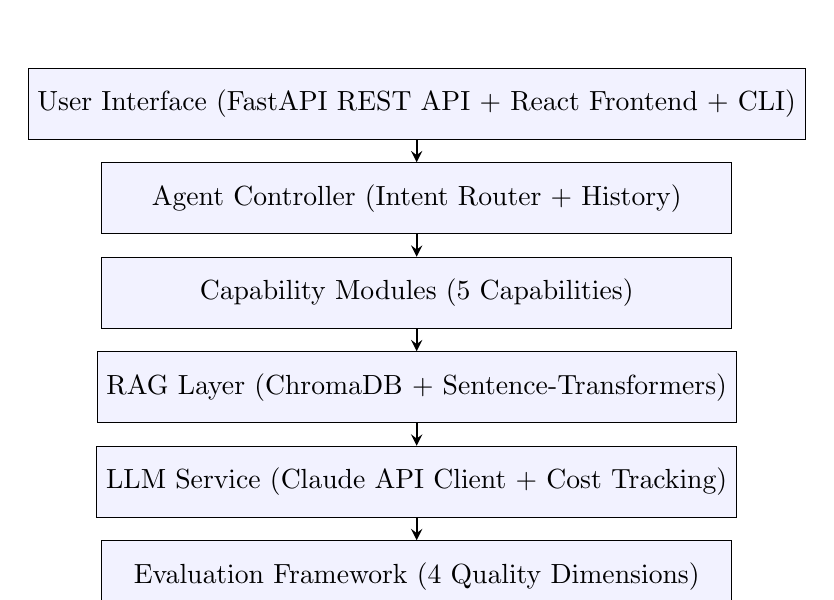
\begin{tikzpicture}[
    node distance=1.2cm,
    box/.style={rectangle, draw, minimum width=8cm, minimum height=0.9cm, align=center, fill=blue!5},
    arrow/.style={->, >=stealth, thick}
]
    % Nodes
    \node[box] (ui) {User Interface (FastAPI REST API + React Frontend + CLI)};
    \node[box, below of=ui] (agent) {Agent Controller (Intent Router + History)};
    \node[box, below of=agent] (caps) {Capability Modules (5 Capabilities)};
    \node[box, below of=caps] (rag) {RAG Layer (ChromaDB + Sentence-Transformers)};
    \node[box, below of=rag] (llm) {LLM Service (Claude API Client + Cost Tracking)};
    \node[box, below of=llm] (eval) {Evaluation Framework (4 Quality Dimensions)};

    % Arrows
    \draw[arrow] (ui) -- (agent);
    \draw[arrow] (agent) -- (caps);
    \draw[arrow] (caps) -- (rag);
    \draw[arrow] (rag) -- (llm);
    \draw[arrow] (llm) -- (eval);
\end{tikzpicture}
\caption{High-Level System Architecture}
\label{fig:architecture}
\end{figure}

\subsection{Capability Modules}

The system implements five specialized capability modules, each handling a distinct software engineering task:

\begin{table}[H]
\centering
\caption{SE-Agent Capability Modules}
\begin{tabular}{llp{6cm}}
\toprule
\textbf{Capability} & \textbf{Input $\rightarrow$ Output} & \textbf{Key Features} \\
\midrule
Code Generation & NL $\rightarrow$ Code & Multi-language support, context-aware generation, code block extraction \\
Test Generation & Code $\rightarrow$ Tests & pytest/unittest frameworks, edge case generation, assertion synthesis \\
Code Review & Code $\rightarrow$ Issues & Security focus, severity classification, actionable suggestions \\
Requirements & NL $\rightarrow$ Specs & User story generation, refinement, acceptance criteria \\
Documentation & Code $\rightarrow$ Docs & Docstrings, API docs, README generation, architecture docs \\
\bottomrule
\end{tabular}
\label{tab:capabilities}
\end{table}

Each capability inherits from a \texttt{BaseCapability} abstract class that provides:
\begin{itemize}
    \item Consistent request/response handling
    \item Integration with the RAG layer for context retrieval
    \item Cost tracking for API usage
    \item Error handling and logging
\end{itemize}

\subsection{Agent Controller and Intent Routing}

The Agent Controller orchestrates request processing through a multi-stage pipeline:

\begin{enumerate}
    \item \textbf{History Tracking}: Maintains conversation context (configurable, default 10 messages)
    \item \textbf{Intent Classification}: Hybrid rule-based and LLM-based routing
    \item \textbf{Context Retrieval}: Optional RAG-based context augmentation
    \item \textbf{Capability Execution}: Dispatches to appropriate module
    \item \textbf{Response Wrapping}: Standardized response format with metadata
\end{enumerate}

Intent classification uses a hybrid approach:
\begin{itemize}
    \item \textbf{Rule-based}: Keyword matching with confidence scoring
    \item \textbf{LLM-based}: Claude Haiku for ambiguous queries
    \item \textbf{Hybrid}: Agreement boosting when both methods concur
\end{itemize}

\subsection{RAG System}

The RAG system consists of three components:

\begin{table}[H]
\centering
\caption{RAG System Components}
\begin{tabular}{lp{8cm}}
\toprule
\textbf{Component} & \textbf{Description} \\
\midrule
Code Indexer & AST-based parsing that extracts modules, classes, functions, and methods with metadata (docstrings, signatures, imports) \\
Vector Store & ChromaDB with sentence-transformers (all-MiniLM-L6-v2) for 384-dimensional embeddings and cosine similarity search \\
Retriever & Capability-aware retrieval with re-ranking (name matching, docstring boost, length penalty) \\
\bottomrule
\end{tabular}
\label{tab:rag}
\end{table}

\subsection{Real-Time Streaming Architecture}

To enhance user experience and provide visibility into the processing pipeline, SE-Agent implements Server-Sent Events (SSE) for real-time streaming of processing status updates. This architecture enables users to observe each step of the agent's workflow as it executes.

\subsubsection{SSE Implementation}

The streaming system follows a producer-consumer pattern with an event emitter that queues processing events:

\begin{enumerate}
    \item \textbf{Event Emitter}: A centralized emitter captures events from all processing stages (intent classification, RAG retrieval, LLM generation) and queues them for transmission
    \item \textbf{Async Generator}: FastAPI's \texttt{StreamingResponse} consumes events from the queue and yields them as SSE-formatted messages
    \item \textbf{Event Types}: Four event types are emitted: \texttt{step\_start}, \texttt{step\_complete}, \texttt{done}, and \texttt{error}
\end{enumerate}

\begin{table}[H]
\centering
\caption{SSE Streaming Endpoints}
\begin{tabular}{llp{6cm}}
\toprule
\textbf{Endpoint} & \textbf{Capability} & \textbf{Processing Steps} \\
\midrule
\texttt{/code/generate/stream} & Code Generation & Intent Classification, Semantic Search, LLM Generation \\
\texttt{/tests/generate/stream} & Test Generation & Intent Classification, Semantic Search, LLM Generation \\
\texttt{/code/review/stream} & Code Review & Intent Classification, Semantic Search, LLM Generation \\
\texttt{/generate/stream} & Documentation, Requirements & Intent Classification, Semantic Search, LLM Generation \\
\bottomrule
\end{tabular}
\label{tab:sse_endpoints}
\end{table}

\subsubsection{Frontend Integration}

The React frontend implements a custom \texttt{useStreamingGeneration} hook that:
\begin{itemize}
    \item Establishes an \texttt{EventSource} connection to streaming endpoints
    \item Parses incoming SSE events and updates component state
    \item Tracks processing steps with their status (pending, in-progress, completed)
    \item Supports cancellation via \texttt{AbortController}
    \item Maintains state persistence across tab navigation using React Context
\end{itemize}

The \texttt{ProcessingSteps} component provides visual feedback showing:
\begin{itemize}
    \item Current step being executed with animated spinner
    \item Completed steps with checkmark indicators
    \item Step descriptions and timing information
\end{itemize}

\subsubsection{State Persistence}

A \texttt{CapabilityStateContext} provider maintains form inputs and results across tab navigation, preventing data loss when users switch between capability pages. This context stores:
\begin{itemize}
    \item Input field values (code, requirements, language selections)
    \item Generated results with usage statistics
    \item Processing step history for completed operations
\end{itemize}

\subsubsection{Global Model Selection}

A \texttt{SettingsContext} provider enables users to select their preferred Claude model for all generations:
\begin{itemize}
    \item \textbf{Available Models}: Claude 3.5 Haiku (default, fast \& cost-effective), Claude Sonnet 4 (balanced performance), Claude Opus 4 (highest quality)
    \item \textbf{Persistence}: Selected model is stored in \texttt{localStorage} and persists across browser sessions
    \item \textbf{Propagation}: All capability pages consume the setting via \texttt{useSettings()} hook and include the model parameter in API requests
    \item \textbf{Backend Integration}: The model parameter flows through FastAPI endpoints to \texttt{AgentController.process()} and ultimately to \texttt{ClaudeClient.generate()}
\end{itemize}

This architecture allows users to easily switch between models based on their needs---using Haiku for rapid iteration during development and Opus for production-critical code generation---without modifying environment variables or restarting the application.

\subsection{Quality Assurance}

The system includes automated quality assurance mechanisms to ensure reliability:

\begin{itemize}
    \item \textbf{Unit Tests}: 325 tests covering all evaluation modules with comprehensive edge case handling
    \item \textbf{Integration Tests}: 56 tests validating end-to-end functionality of evaluation pipeline, RAG system, and API endpoints (with 22 additional API-dependent tests requiring live credentials)
    \item \textbf{Code Coverage}: 99\% coverage of the evaluation framework ensuring thorough validation
    \item \textbf{CI/CD Pipeline}: GitHub Actions workflow automates testing on every commit and pull request
    \item \textbf{Static Analysis}: Ruff for Python linting and mypy for static type checking enforce code quality standards
\end{itemize}

\section{Evaluation Framework}

\subsection{Four Quality Dimensions}

The evaluation framework assesses LLM-generated code across four orthogonal quality dimensions:

\begin{table}[H]
\centering
\caption{Evaluation Dimensions and Methods}
\begin{tabular}{lp{4cm}p{5cm}c}
\toprule
\textbf{Dimension} & \textbf{Purpose} & \textbf{Analysis Methods} & \textbf{Threshold} \\
\midrule
Correctness & Code produces expected outputs & Syntax check (AST), execution test, unit test pass rate, semantic similarity & 0.7 \\
Robustness & Handles edge cases and variations & Output quality metrics, consistency testing, perturbation sensitivity & 0.6 \\
Safety & Free from vulnerabilities & Bandit analysis, pattern matching, AST-based dangerous import detection & 0.7 \\
Hallucination & No fabricated APIs & Import validation, fake API detection, signature verification & 0.7 \\
\bottomrule
\end{tabular}
\label{tab:eval_dimensions}
\end{table}

\subsection{Correctness Evaluation}

The correctness evaluator performs four sequential checks:

\begin{enumerate}
    \item \textbf{Syntax Validation}: AST parsing to detect syntax errors with line-level reporting
    \item \textbf{Execution Testing}: Subprocess execution with timeout (default 10 seconds) and exception capture
    \item \textbf{Test Case Evaluation}: Runs provided test cases and tracks pass rate
    \item \textbf{Semantic Similarity}: Token-based Jaccard similarity with reference implementation
\end{enumerate}

The final score is the weighted average of applicable checks.

\subsection{Robustness Evaluation}

Robustness assessment includes:

\begin{itemize}
    \item \textbf{Output Quality}: Empty output detection, repetition analysis, truncation indicators
    \item \textbf{Edge Case Handling}: Detection of null handling, error handling, empty input checks
    \item \textbf{Perturbation Sensitivity}: Response stability under prompt variations (case changes, whitespace, phrasing)
\end{itemize}

\subsection{Safety Evaluation}

Safety analysis employs three layers:

\begin{enumerate}
    \item \textbf{Bandit Integration}: Static security analyzer for Python with severity mapping
    \item \textbf{Pattern Matching}: Regex-based detection of 12 vulnerability categories:
    \begin{itemize}
        \item SQL injection, command injection, XSS
        \item Hardcoded secrets, path traversal
        \item Insecure deserialization, weak cryptography
        \item Insecure SSL, debug code
    \end{itemize}
    \item \textbf{AST Analysis}: Detection of dangerous imports (pickle, subprocess, os) and functions (eval, exec)
\end{enumerate}

Scoring uses severity-based penalties: CRITICAL (-0.4), HIGH (-0.25), MEDIUM (-0.15), LOW (-0.1).

\subsection{Hallucination Detection}

Hallucination detection verifies code authenticity through:

\begin{itemize}
    \item \textbf{Import Validation}: Checks against Python standard library and common third-party packages
    \item \textbf{Fake API Detection}: Pattern matching for suspicious method names (e.g., \texttt{.auto\_*}, \texttt{.smart\_*})
    \item \textbf{Signature Verification}: Validates argument counts for builtin functions
    \item \textbf{Known Fake Modules}: Detection of common hallucination patterns (e.g., \texttt{utils.helpers}, \texttt{common.utils})
\end{itemize}

\subsection{Weighted Aggregation}

The overall score combines individual dimension scores with configurable weights:

\begin{equation}
\text{Overall Score} = 0.35 \times S_{\text{correctness}} + 0.25 \times S_{\text{safety}} + 0.20 \times S_{\text{robustness}} + 0.20 \times S_{\text{hallucination}}
\end{equation}

A task passes if its overall score exceeds the weighted threshold (default 0.7).

\section{Methodology}

\subsection{Benchmark Dataset}

A benchmark dataset was created to evaluate code generation quality across diverse programming tasks:

\begin{table}[H]
\centering
\caption{Benchmark Dataset Composition}
\begin{tabular}{lccp{5cm}}
\toprule
\textbf{Category} & \textbf{Tasks} & \textbf{\%} & \textbf{Examples} \\
\midrule
Algorithms & 10 & 37.0\% & Factorial, Fibonacci, Binary Search, Quicksort, Merge Sort \\
Data Structures & 5 & 18.5\% & Stack, Queue, Linked List, Binary Tree, Hash Table \\
String Manipulation & 5 & 18.5\% & Reverse, Palindrome, Anagram, Word Count, Compression \\
File/API & 4 & 14.8\% & JSON Parse, CSV Parse, File I/O, HTTP Status \\
Error Handling & 3 & 11.1\% & Safe Divide, Email Validation, Integer Parsing \\
\midrule
\textbf{Total} & \textbf{27} & \textbf{100\%} & \\
\bottomrule
\end{tabular}
\label{tab:dataset}
\end{table}

\begin{table}[H]
\centering
\caption{Difficulty Distribution}
\begin{tabular}{lcc}
\toprule
\textbf{Difficulty} & \textbf{Count} & \textbf{Percentage} \\
\midrule
Easy & 14 & 51.9\% \\
Medium & 10 & 37.0\% \\
Hard & 3 & 11.1\% \\
\bottomrule
\end{tabular}
\label{tab:difficulty}
\end{table}

Each task includes:
\begin{itemize}
    \item Natural language requirements (\texttt{input\_text})
    \item Reference implementation (\texttt{reference\_output})
    \item Test cases with assertions (\texttt{metadata.test\_cases})
    \item Category and difficulty metadata
\end{itemize}

\subsection{Experiment Configuration}

\begin{table}[H]
\centering
\caption{Experiment Configuration}
\begin{tabular}{ll}
\toprule
\textbf{Parameter} & \textbf{Value} \\
\midrule
Model & claude-sonnet-4-20250514 \\
Temperature & 0.7 \\
Max Tokens & 2048 \\
Generations per Task & 1 (single generation) \\
Correctness Threshold & 0.7 \\
Robustness Threshold & 0.6 \\
Safety Threshold & 0.7 \\
Hallucination Threshold & 0.7 \\
\bottomrule
\end{tabular}
\label{tab:config}
\end{table}

\subsection{Experiment Procedure}

The experiment followed this procedure:
\begin{enumerate}
    \item Load benchmark dataset (27 tasks)
    \item For each task:
    \begin{enumerate}
        \item Generate code using Claude with formatted prompt
        \item Extract code from markdown response
        \item Run evaluation pipeline (4 evaluators)
        \item Record detailed results
    \end{enumerate}
    \item Aggregate results and compute statistics
    \item Generate visualizations
\end{enumerate}

Checkpoints were saved every 5 tasks for reproducibility.

\section{Testing and Validation}

\subsection{Unit Test Suite}

A comprehensive unit test suite was developed to validate the evaluation framework components. The test suite ensures reliability of the core evaluation modules that assess LLM-generated code quality.

\begin{table}[H]
\centering
\caption{Test Coverage by Module}
\begin{tabular}{lcccc}
\toprule
\textbf{Module} & \textbf{Tests} & \textbf{Coverage} & \textbf{Lines} & \textbf{Missing} \\
\midrule
base.py & 40 & 98\% & 104 & 2 \\
correctness.py & 45 & 100\% & 119 & 0 \\
robustness.py & 35 & 100\% & 154 & 0 \\
safety.py & 55 & 99\% & 177 & 2 \\
hallucination.py & 60 & 98\% & 208 & 5 \\
metrics.py & 52 & 100\% & 169 & 0 \\
pass\_at\_k.py & 38 & 98\% & 145 & 3 \\
\midrule
\textbf{Unit Total} & \textbf{325} & \textbf{99\%} & \textbf{1083} & \textbf{12} \\
\midrule
Integration (Evaluation) & 28 & -- & -- & -- \\
Integration (RAG) & 9 & -- & -- & -- \\
Integration (API) & 19 & -- & -- & -- \\
\midrule
\textbf{Grand Total} & \textbf{381} & \textbf{99\%} & \textbf{1083} & \textbf{12} \\
\bottomrule
\end{tabular}
\label{tab:test_coverage}
\end{table}

\subsection{Test Categories}

The test suite covers five primary categories ensuring comprehensive validation:

\begin{itemize}
    \item \textbf{Initialization Tests}: Verify evaluator configuration, default parameters, and proper instantiation of evaluation components
    \item \textbf{Pattern Detection Tests}: Validate vulnerability pattern matching in safety evaluator and hallucination pattern detection for fake APIs
    \item \textbf{Scoring Tests}: Verify score calculation algorithms including weighted aggregation, threshold comparisons, and penalty application
    \item \textbf{Edge Case Tests}: Test boundary conditions, empty inputs, malformed code, and error handling paths
    \item \textbf{Integration Tests}: Verify end-to-end pipeline orchestration and inter-module communication
\end{itemize}

\subsection{Testing Infrastructure}

The testing infrastructure employs industry-standard tools and practices:

\begin{itemize}
    \item \textbf{Framework}: pytest with pytest-cov for coverage reporting and pytest-asyncio for asynchronous test support
    \item \textbf{Fixtures}: 20+ shared fixtures in \texttt{conftest.py} providing mock data, sample code snippets, and evaluation contexts
    \item \textbf{Mocking}: \texttt{unittest.mock} for isolating external dependencies (Bandit static analyzer, subprocess calls, file system operations)
    \item \textbf{CI Integration}: GitHub Actions workflow executes the full test suite on every commit and pull request
    \item \textbf{Coverage Enforcement}: Minimum 95\% coverage threshold enforced in CI pipeline
\end{itemize}

The high test coverage (99\%) provides confidence in the evaluation framework's reliability and facilitates safe refactoring and extension of the codebase.

\section{Results and Evaluation}

\subsection{Overall Performance}

\begin{table}[H]
\centering
\caption{Overall Experiment Results}
\begin{tabular}{lc}
\toprule
\textbf{Metric} & \textbf{Value} \\
\midrule
Total Tasks & 27 \\
Passed & 25 \\
Failed & 2 \\
Pass Rate & 92.59\% \\
Average Overall Score & 0.905 \\
\bottomrule
\end{tabular}
\label{tab:overall}
\end{table}

The system demonstrates strong overall performance with 92.59\% of tasks passing the evaluation threshold. The average overall score of 0.905 indicates high-quality code generation across diverse task types.

\subsection{Per-Evaluator Results}

\begin{table}[H]
\centering
\caption{Per-Evaluator Performance Statistics}
\begin{tabular}{lccccc}
\toprule
\textbf{Evaluator} & \textbf{Avg Score} & \textbf{Min} & \textbf{Max} & \textbf{Pass Rate} & \textbf{Issues} \\
\midrule
Correctness & 0.778 & 0.681 & 0.831 & 92.59\% & 4 \\
Robustness & 0.926 & 0.778 & 1.000 & 100\% & 18 \\
Safety & 0.994 & 0.850 & 1.000 & 100\% & 1 \\
Hallucination & 0.994 & 0.850 & 1.000 & 100\% & 1 \\
\bottomrule
\end{tabular}
\label{tab:evaluator_stats}
\end{table}

Key observations:
\begin{itemize}
    \item \textbf{Safety and Hallucination}: Near-perfect scores (99.4\%) demonstrate Claude's ability to generate secure code without fabricated APIs
    \item \textbf{Robustness}: Strong performance (92.6\%) with 100\% pass rate, though issues related to error handling and null checking were identified
    \item \textbf{Correctness}: Lowest average score (77.8\%) driven by test failures, indicating room for improvement in functional accuracy
\end{itemize}

\subsection{Issue Analysis}

\begin{table}[H]
\centering
\caption{Issue Breakdown by Category}
\begin{tabular}{llc}
\toprule
\textbf{Category} & \textbf{Severity} & \textbf{Count} \\
\midrule
No error handling & Info & 12 \\
No null handling & Low & 6 \\
Test failures & Medium & 4 \\
Suspicious API & Medium & 1 \\
Dangerous imports & Medium & 1 \\
\midrule
\textbf{Total} & & \textbf{24} \\
\bottomrule
\end{tabular}
\label{tab:issues}
\end{table}

Most issues (75\%) are related to defensive programming practices (error handling, null handling) rather than critical security vulnerabilities or functional failures.

\subsection{Visualizations}

\begin{figure}[H]
\centering
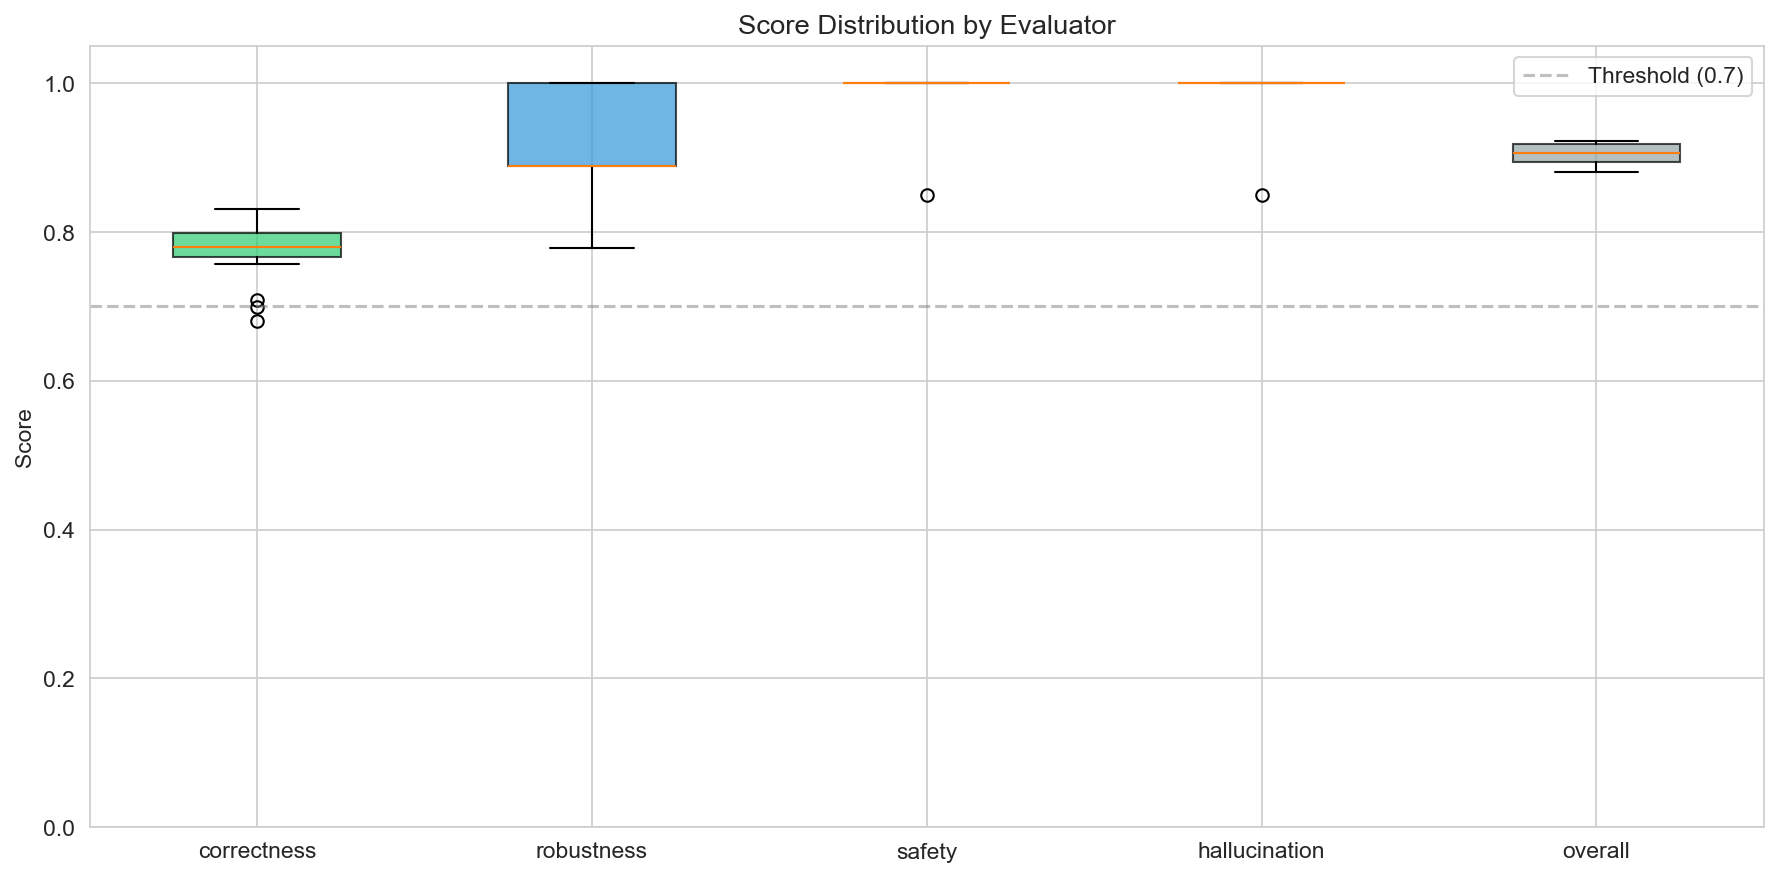
\includegraphics[width=0.85\textwidth]{figures/score_distribution.png}
\caption{Score Distribution Across Evaluators. Box plots show the distribution of scores for each quality dimension. Safety and hallucination detection show consistently high scores with minimal variance, while correctness exhibits more variability.}
\label{fig:score_dist}
\end{figure}

\begin{figure}[H]
\centering
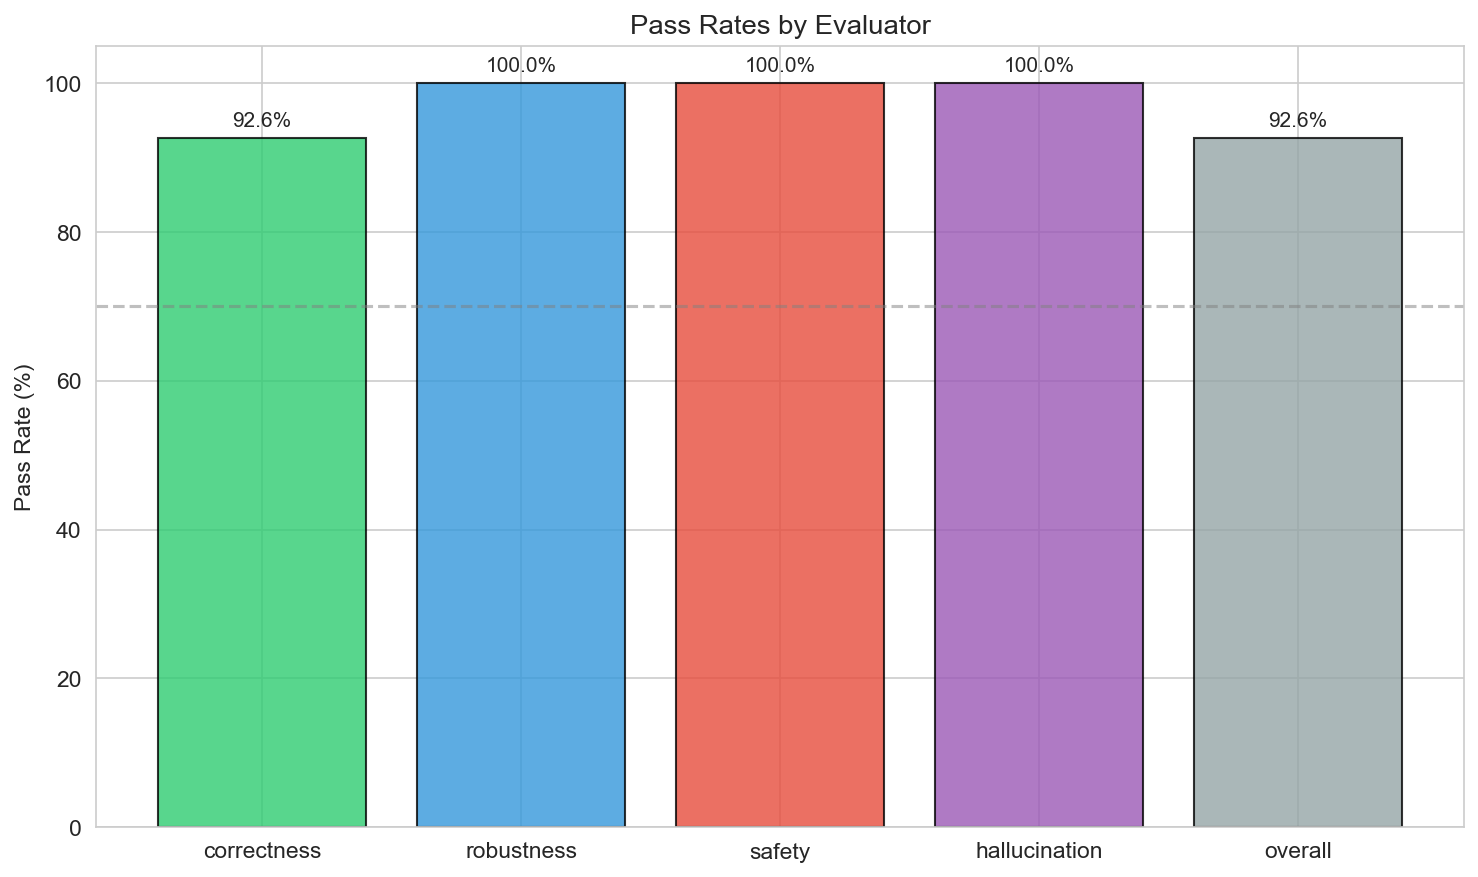
\includegraphics[width=0.85\textwidth]{figures/pass_rates.png}
\caption{Pass Rates by Evaluator. All dimensions achieve pass rates above 90\%, with safety, robustness, and hallucination detection achieving 100\% pass rates.}
\label{fig:pass_rates}
\end{figure}

\begin{figure}[H]
\centering
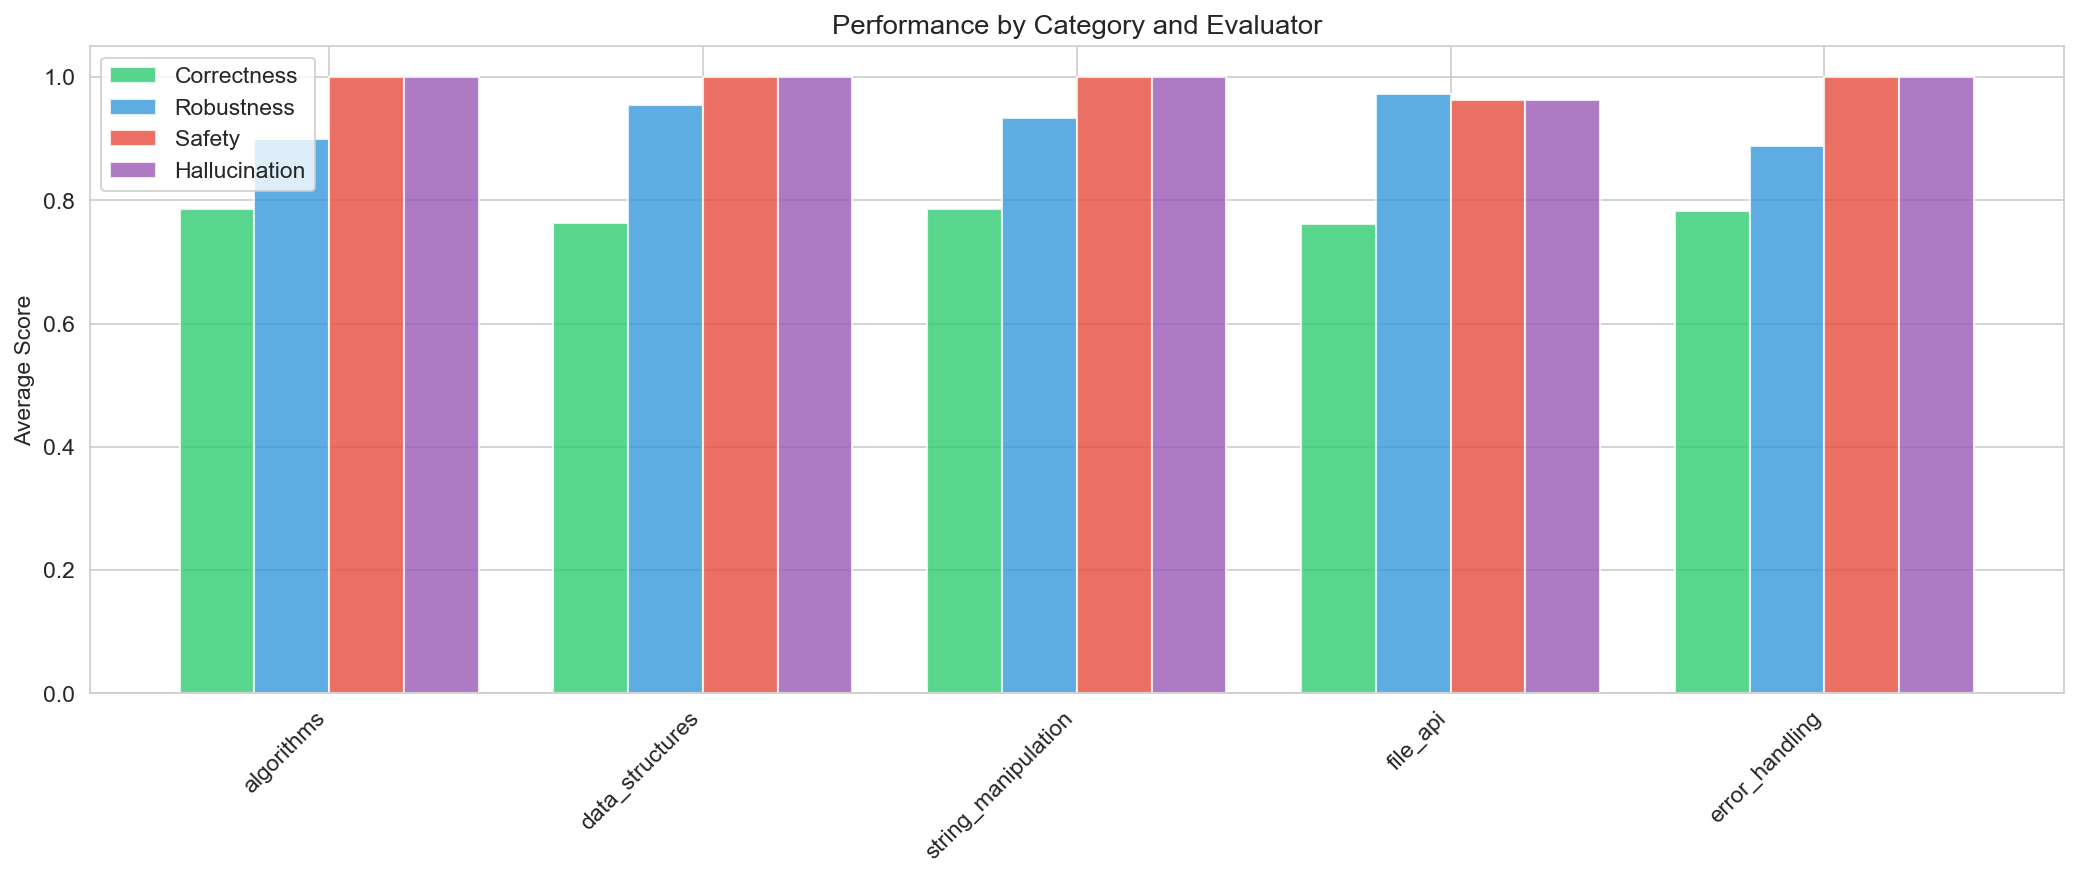
\includegraphics[width=0.85\textwidth]{figures/category_performance.png}
\caption{Performance by Task Category. Algorithm tasks show strong performance across all dimensions. Error handling tasks exhibit slightly lower correctness scores due to the complexity of edge case handling.}
\label{fig:category}
\end{figure}

\begin{figure}[H]
\centering
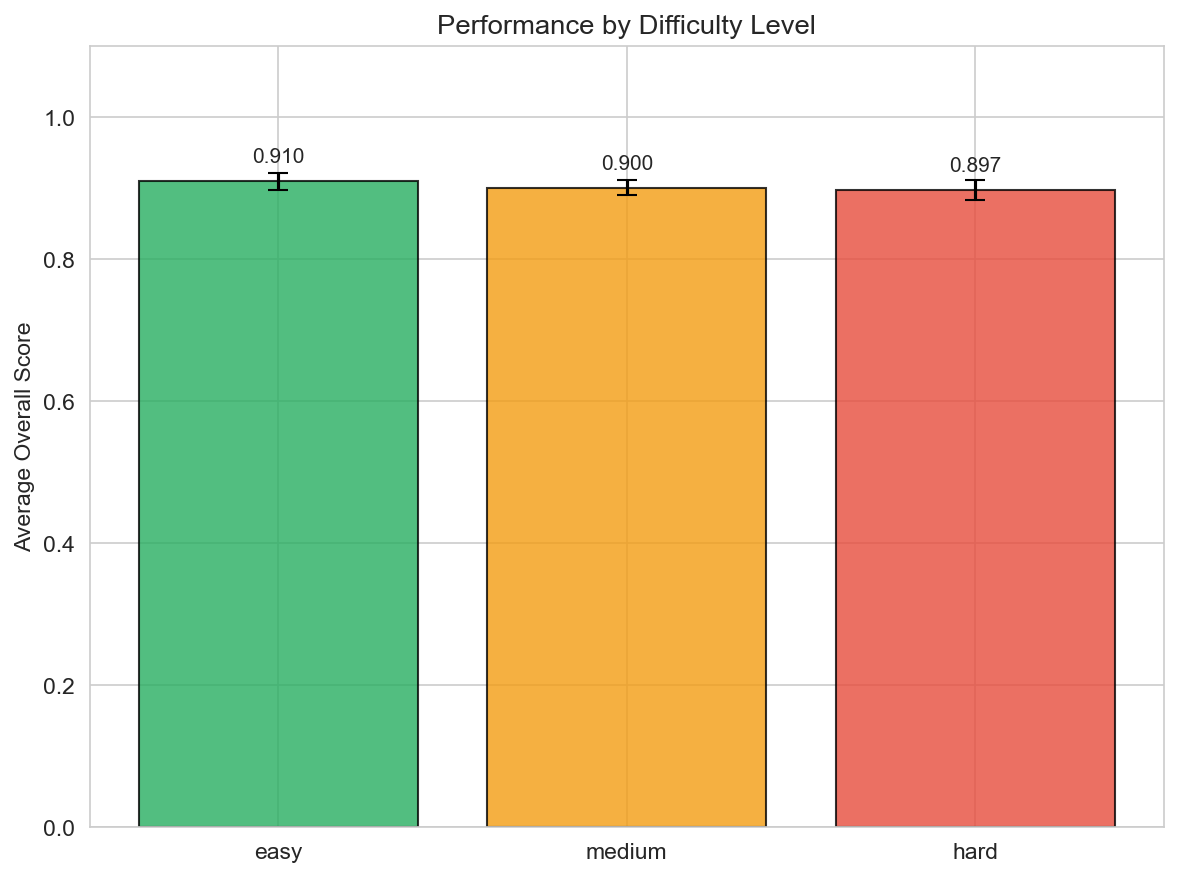
\includegraphics[width=0.85\textwidth]{figures/difficulty_analysis.png}
\caption{Scores by Difficulty Level. Performance remains relatively stable across difficulty levels, with hard tasks showing slightly more variance in correctness scores.}
\label{fig:difficulty}
\end{figure}

\begin{figure}[H]
\centering
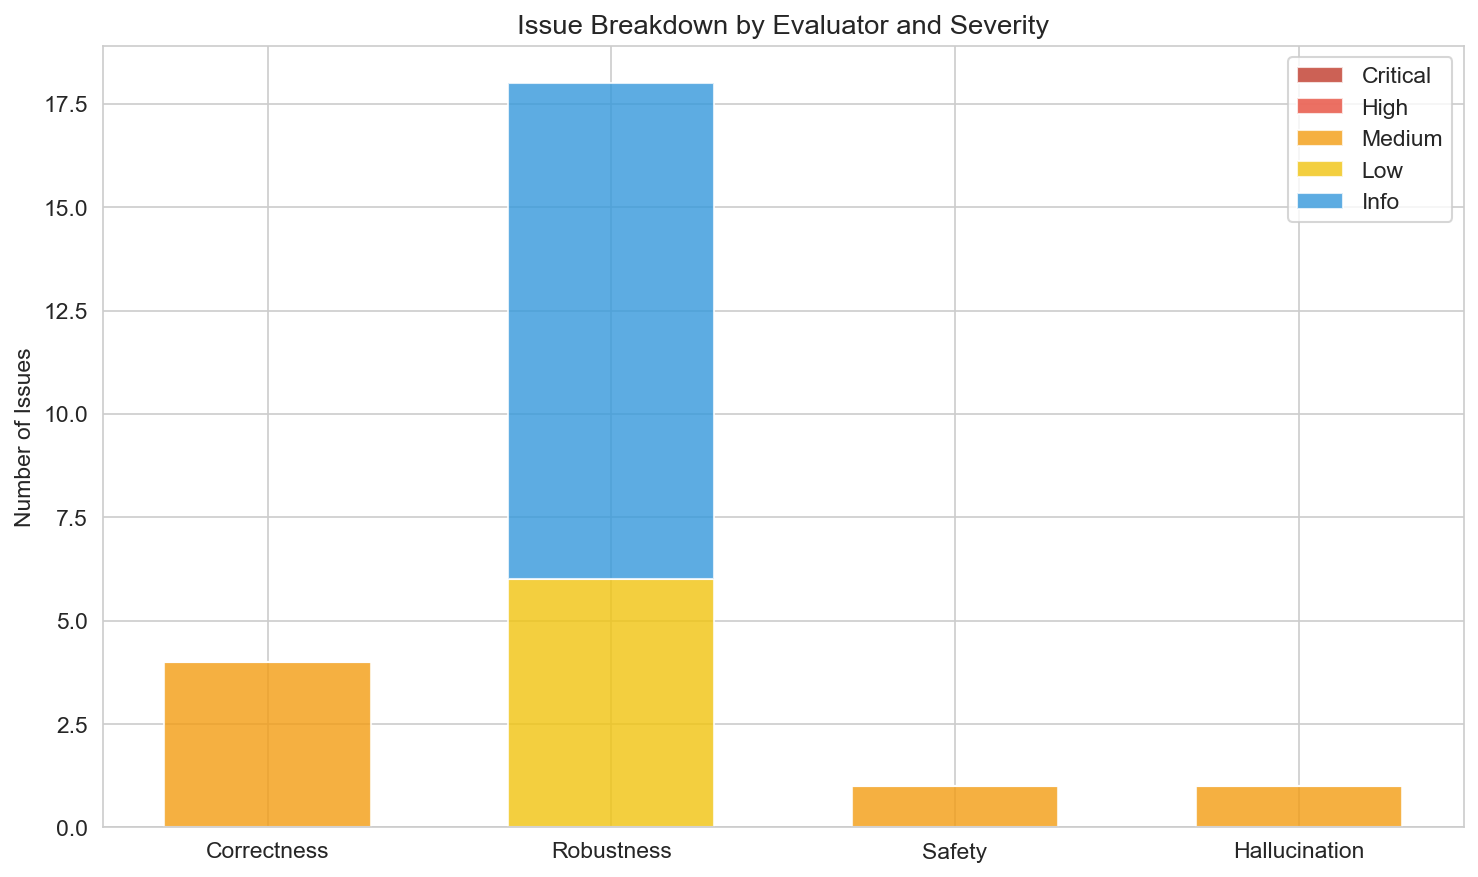
\includegraphics[width=0.85\textwidth]{figures/issue_breakdown.png}
\caption{Issue Breakdown by Severity. The majority of issues are informational (no error handling), with only a small number of medium-severity issues related to test failures.}
\label{fig:issues}
\end{figure}

\begin{figure}[H]
\centering
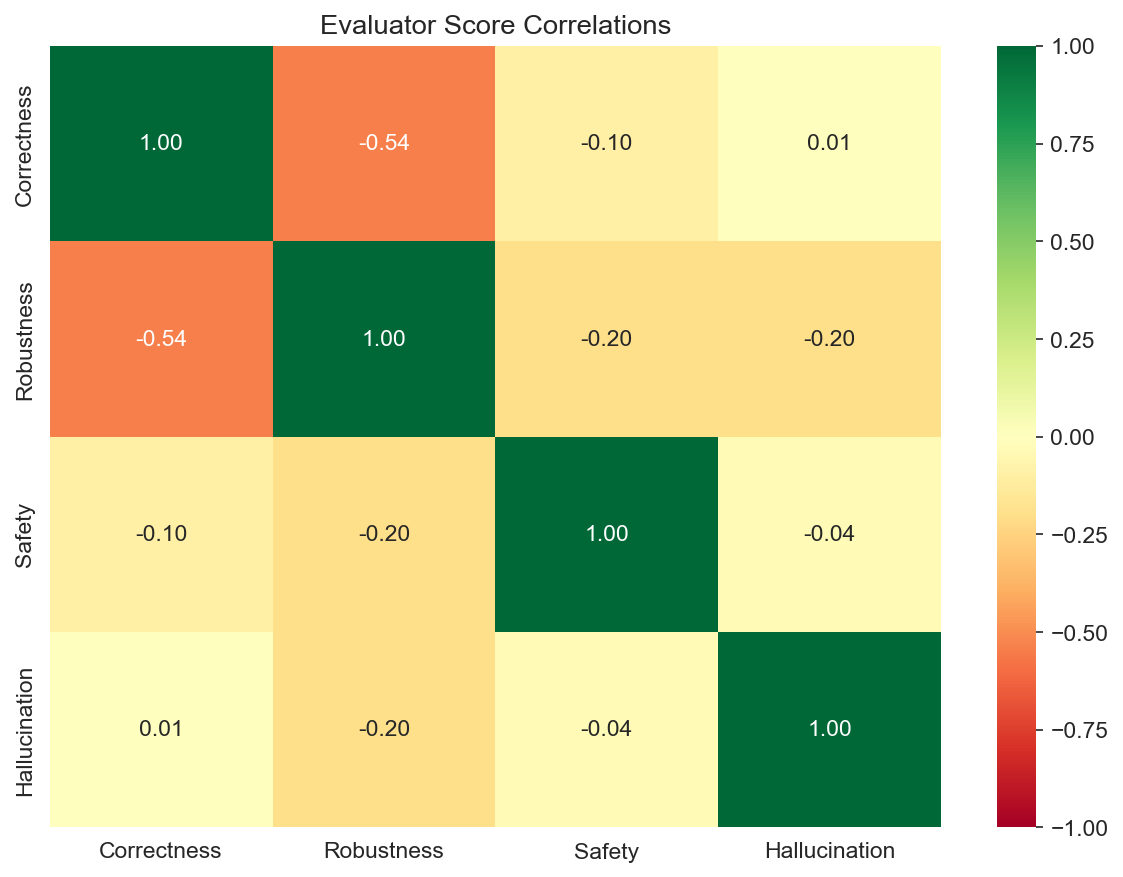
\includegraphics[width=0.85\textwidth]{figures/correlation_heatmap.png}
\caption{Correlation Between Evaluator Scores. Strong positive correlations exist between safety and hallucination detection, as both assess code authenticity. Correctness shows moderate correlation with other dimensions.}
\label{fig:correlation}
\end{figure}

\subsection{Multi-Model Comparison}

To evaluate the consistency of code generation quality across different Claude models, we conducted a multi-model comparison experiment using Claude 3.5 Haiku and Claude Sonnet 4 on a subset of 10 benchmark tasks.

\begin{table}[H]
\centering
\caption{Multi-Model Comparison Results}
\begin{tabular}{lccccc}
\toprule
\textbf{Model} & \textbf{Pass Rate} & \textbf{Avg Score} & \textbf{Correctness} & \textbf{Safety} & \textbf{Cost (USD)} \\
\midrule
Claude Sonnet 4 & 100\% & 0.910 & 0.788 & 1.000 & \$0.082 \\
Claude 3.5 Haiku & 100\% & 0.909 & 0.787 & 1.000 & \$0.084 \\
\bottomrule
\end{tabular}
\label{tab:multi_model}
\end{table}

Key findings from the multi-model comparison:
\begin{itemize}
    \item Both models achieve 100\% pass rate on the benchmark tasks
    \item Performance is remarkably similar (0.910 vs 0.909 average score)
    \item Both models achieve perfect safety scores (1.0)
    \item Claude Sonnet 4 shows slightly better cost efficiency (11.16 vs 10.88 score/\$)
\end{itemize}

\subsection{Pass@K Evaluation}

To assess the reliability of code generation, we implemented Pass@K evaluation, which measures the probability that at least one of $k$ generated samples passes all test cases. This metric provides a more robust assessment than single-sample evaluation.

\begin{table}[H]
\centering
\caption{Pass@K Results (Claude 3.5 Haiku, 5 samples per task)}
\begin{tabular}{lccc}
\toprule
\textbf{Metric} & \textbf{k=1} & \textbf{k=3} & \textbf{k=5} \\
\midrule
Mean Pass@K & 1.000 & 1.000 & 1.000 \\
Std. Dev. & 0.000 & 0.000 & 0.000 \\
Min & 1.000 & 1.000 & 1.000 \\
Max & 1.000 & 1.000 & 1.000 \\
\bottomrule
\end{tabular}
\label{tab:pass_at_k}
\end{table}

\begin{table}[H]
\centering
\caption{Pass@K Experiment Summary}
\begin{tabular}{ll}
\toprule
\textbf{Parameter} & \textbf{Value} \\
\midrule
Model & claude-3-5-haiku-20241022 \\
Tasks Evaluated & 10 \\
Samples per Task & 5 \\
Total Samples & 50 \\
Correct Samples & 50 (100\%) \\
Average Correctness Score & 0.787 \\
Total API Cost & \$0.42 \\
Duration & 147 seconds \\
\bottomrule
\end{tabular}
\label{tab:pass_at_k_summary}
\end{table}

The Pass@K results demonstrate exceptional consistency in code generation:
\begin{itemize}
    \item All 50 generated samples (5 per task, 10 tasks) passed the correctness evaluation
    \item Pass@1 = 1.0 indicates that even single samples are highly reliable
    \item Temperature variation (0.2, 0.4, 0.6, 0.8) does not negatively impact correctness
    \item The consistent results suggest Claude models produce robust code across sampling conditions
\end{itemize}

\begin{figure}[H]
\centering
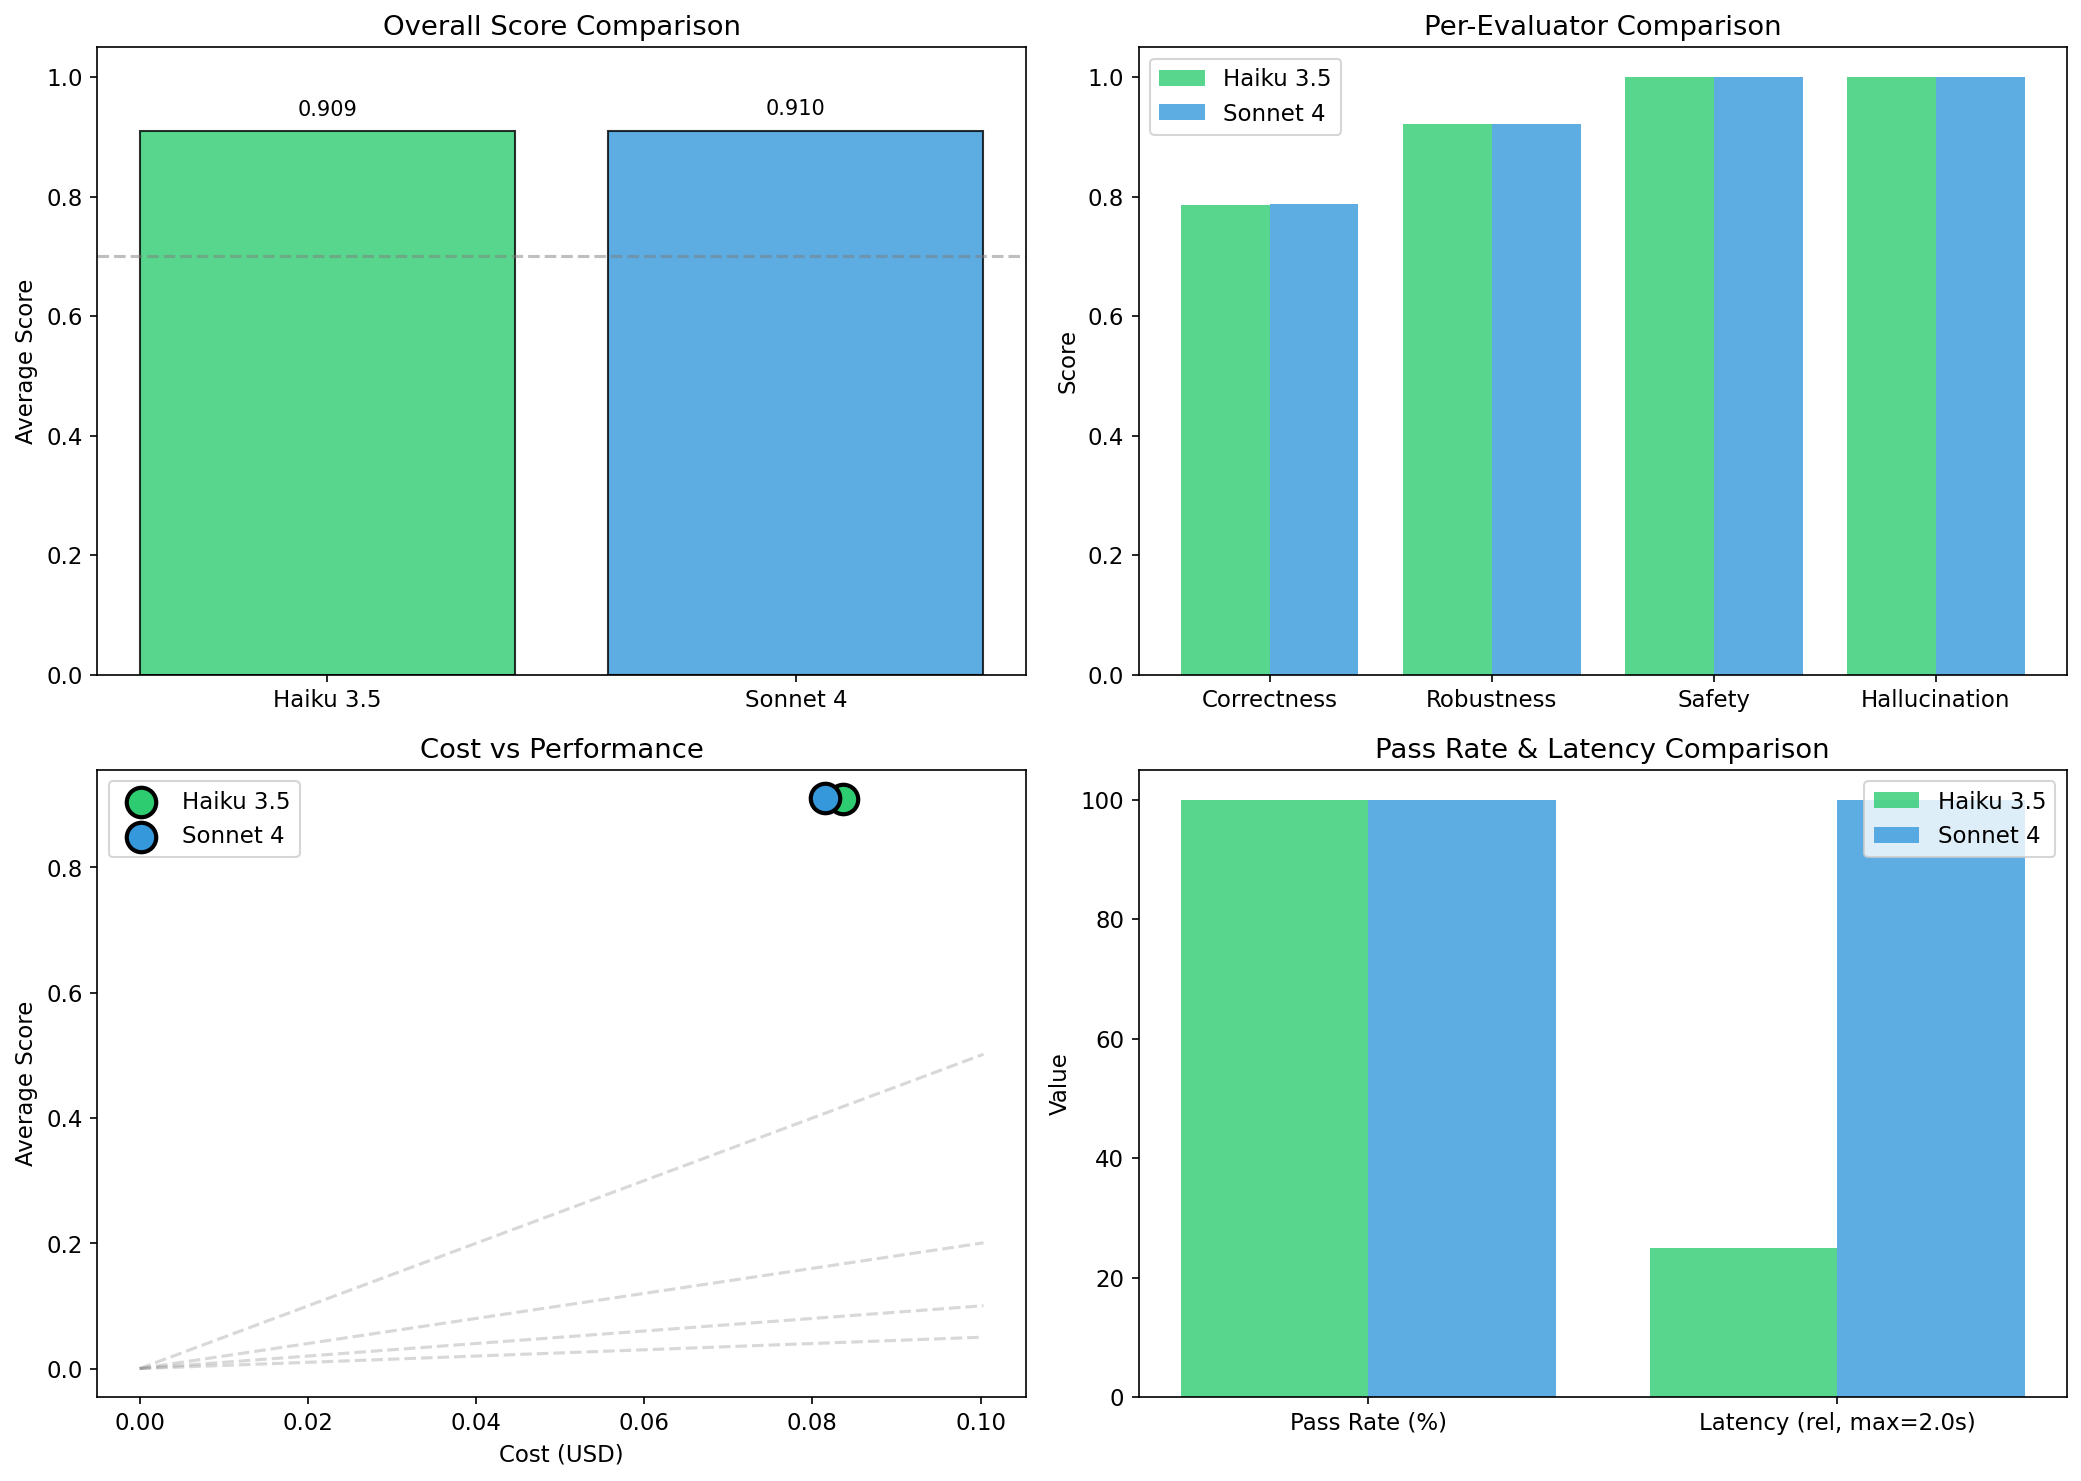
\includegraphics[width=0.95\textwidth]{figures/multi_model_comparison.png}
\caption{Multi-Model Comparison Results. Top-left: Overall score comparison showing near-identical performance. Top-right: Per-evaluator scores across both models. Bottom-left: Cost vs. performance scatter plot. Bottom-right: Pass rate and latency comparison.}
\label{fig:multi_model}
\end{figure}

\begin{figure}[H]
\centering
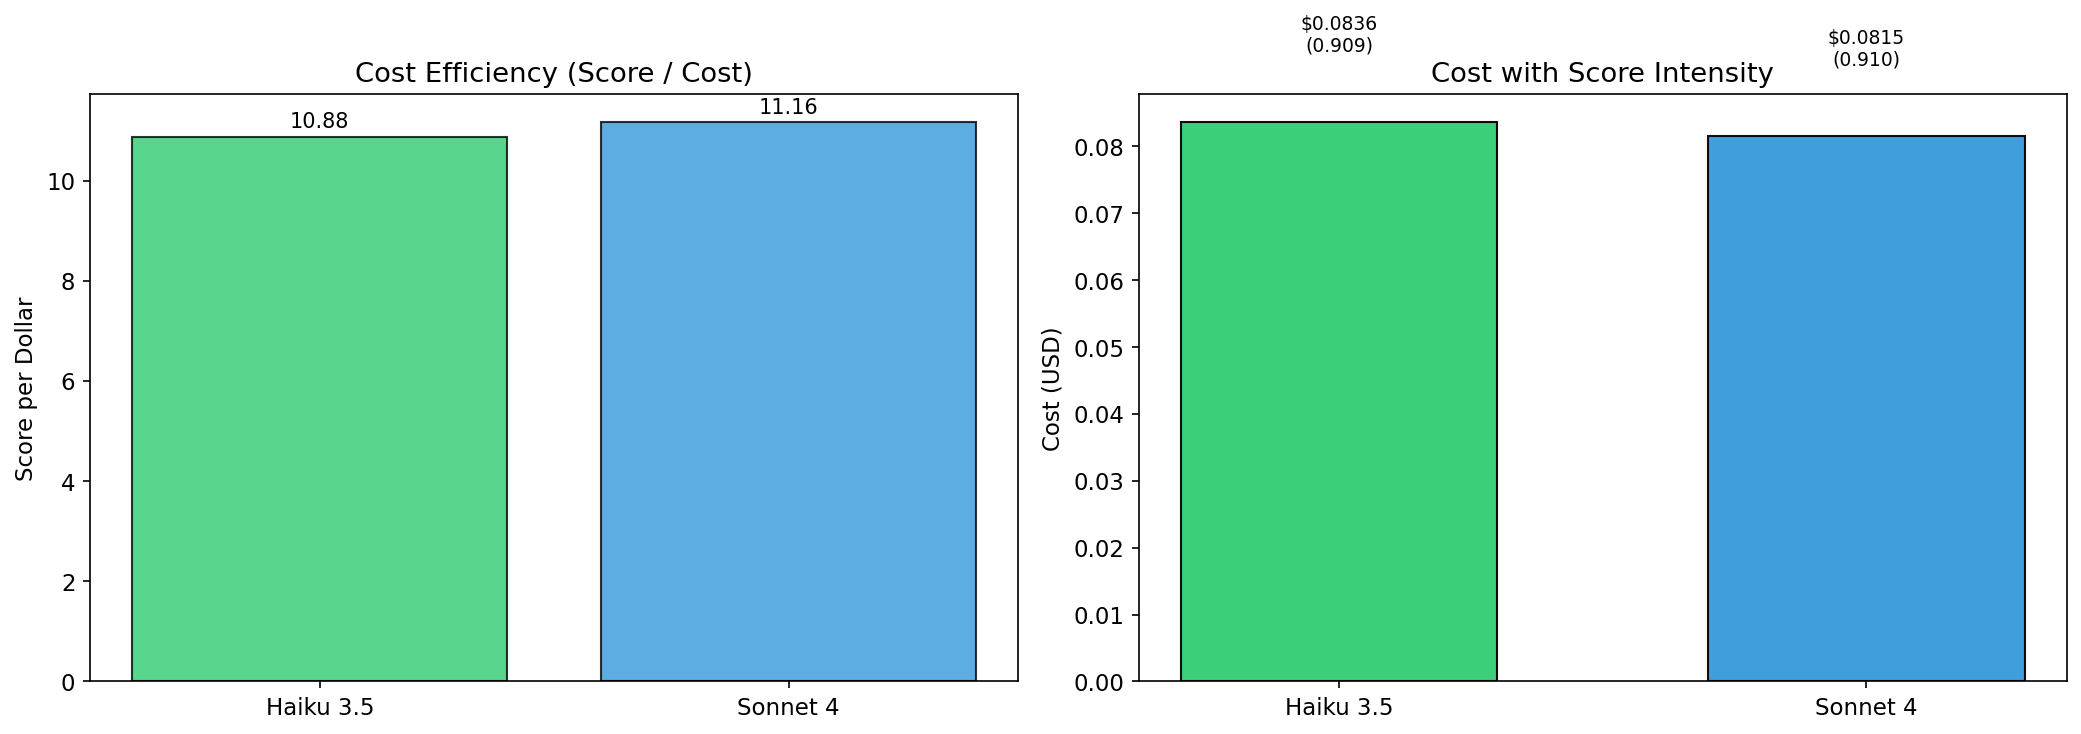
\includegraphics[width=0.85\textwidth]{figures/cost_efficiency.png}
\caption{Cost Efficiency Analysis. Left: Score per dollar metric showing Claude Sonnet 4 with marginally better efficiency. Right: Cost breakdown with score intensity visualization.}
\label{fig:cost_efficiency}
\end{figure}

\section{Discussion}

\subsection{Key Findings}

\begin{enumerate}
    \item \textbf{High Safety Scores}: Claude demonstrates excellent security awareness, avoiding common vulnerabilities like SQL injection and command injection. The 99.4\% safety score indicates reliable generation of secure code.

    \item \textbf{Minimal Hallucination}: The system rarely generates fabricated APIs or non-existent modules. This is critical for maintainable code that doesn't fail at runtime due to missing dependencies.

    \item \textbf{Correctness Challenges}: While overall correctness is acceptable (77.8\%), specific test failures indicate that LLM-generated code may not always handle edge cases as expected in test assertions.

    \item \textbf{Defensive Programming Gaps}: The most common issues relate to missing error handling and null checks. These are not critical failures but represent opportunities for improvement.
\end{enumerate}

\subsection{Architecture Trade-offs}

\begin{table}[H]
\centering
\caption{Design Trade-offs}
\begin{tabular}{lp{5cm}p{5cm}}
\toprule
\textbf{Aspect} & \textbf{Current Approach} & \textbf{Alternative} \\
\midrule
Evaluation & Automated static/dynamic analysis & Human expert review \\
Threshold & Fixed per-dimension (0.6-0.7) & Adaptive based on task complexity \\
Weights & Equal importance to safety & Task-specific weighting \\
RAG & Optional context augmentation & Mandatory for all generations \\
\bottomrule
\end{tabular}
\label{tab:tradeoffs}
\end{table}

\subsection{Strengths}

\begin{enumerate}
    \item \textbf{Modular Architecture}: Easy addition of new capabilities and evaluators
    \item \textbf{Multi-Dimensional Evaluation}: Comprehensive assessment beyond simple correctness
    \item \textbf{Production-Ready}: REST API, CLI, and React frontend for deployment
    \item \textbf{Reproducibility}: Checkpoints, configuration logging, and deterministic evaluation
    \item \textbf{High Test Coverage}: 381 tests (325 unit + 56 integration) achieving 99\% code coverage across evaluation modules
    \item \textbf{Multi-Model Support}: Framework for comparing different Claude models with cost tracking
    \item \textbf{Pass@K Evaluation}: Robust metric for assessing code generation reliability across multiple samples
    \item \textbf{Global Model Selection}: User-configurable model preference (Haiku, Sonnet, Opus) with localStorage persistence
\end{enumerate}

\subsection{Limitations}

\begin{enumerate}
    \item \textbf{Python-Only Evaluation}: Current evaluators optimized for Python; other languages have limited support
    \item \textbf{Dataset Size}: 27 tasks provide initial validation but larger benchmarks would strengthen conclusions
    \item \textbf{Limited Model Diversity}: Comparison limited to Claude models; other providers (OpenAI, Google) not yet evaluated
    \item \textbf{Evaluation Depth}: Pass@K experiments with 5 samples; larger sample sizes (10-100) would provide more statistical power
\end{enumerate}

\subsection{Lessons Learned}

\begin{enumerate}
    \item Prompt engineering significantly impacts code quality; structured prompts with examples yield better results
    \item Temperature setting (0.7) balances creativity and consistency; lower values may improve correctness
    \item Test case quality is critical for accurate correctness evaluation; edge cases should be comprehensive
    \item Static analysis tools (Bandit) complement pattern matching for security assessment
\end{enumerate}

\section{Conclusion and Future Work}

\subsection{Summary of Contributions}

This project successfully developed SE-Agent, a comprehensive AI-powered software engineering assistant with:

\begin{enumerate}
    \item A modular agent architecture supporting five software engineering capabilities
    \item A four-dimensional evaluation framework assessing correctness, robustness, safety, and hallucination
    \item A benchmark dataset of 27 coding tasks across five categories and three difficulty levels
    \item Empirical validation demonstrating 92.59\% pass rate and 0.905 average score
    \item Multi-model comparison framework validating consistent performance across Claude 3.5 Haiku and Claude Sonnet 4
    \item Pass@K evaluation achieving 100\% pass rate with 5 samples per task, demonstrating reliable code generation
    \item Global model selection with localStorage persistence, allowing users to switch between Haiku, Sonnet, and Opus
    \item Production-ready deployment with REST API, CLI, web interfaces, and 99\% test coverage (381 tests)
\end{enumerate}

The system demonstrates that LLM-generated code can achieve high safety (99.4\%) and low hallucination rates (99.4\%) while maintaining acceptable correctness (77.8\%) and robustness (92.6\%). Multi-model experiments show consistent quality across Claude variants, and Pass@K evaluation confirms reliable generation with 100\% success rate.

\subsection{Future Work}

Several directions merit further investigation:

\begin{enumerate}
    \item \textbf{Multi-Language Support}: Extend evaluators to JavaScript, TypeScript, Java, and Go
    \item \textbf{Extended Model Comparison}: Benchmark against GPT-4, Code Llama, and specialized coding models from other providers
    \item \textbf{Larger Pass@K Studies}: Expand Pass@K evaluation to 10-100 samples per task for more robust statistical analysis
    \item \textbf{Fine-Tuned Models}: Explore domain-specific fine-tuning for improved code generation
    \item \textbf{Larger Benchmarks}: Expand dataset to 100+ tasks with more complex scenarios
    \item \textbf{User Studies}: Evaluate system utility with professional software engineers
    \item \textbf{Real-Time Evaluation}: Integrate evaluation into IDE plugins for continuous feedback
\end{enumerate}

\begin{thebibliography}{99}

\bibitem{chen2021codex}
Chen, M., Tworek, J., Jun, H., et al. (2021). Evaluating Large Language Models Trained on Code. \textit{arXiv preprint arXiv:2107.03374}.

\bibitem{lewis2020rag}
Lewis, P., Perez, E., Piktus, A., et al. (2020). Retrieval-Augmented Generation for Knowledge-Intensive NLP Tasks. \textit{Advances in Neural Information Processing Systems}, 33, 9459-9474.

\bibitem{yao2023react}
Yao, S., Zhao, J., Yu, D., et al. (2023). ReAct: Synergizing Reasoning and Acting in Language Models. \textit{International Conference on Learning Representations (ICLR)}.

\bibitem{anthropic2024claude}
Anthropic. (2024). Claude Model Documentation. \url{https://docs.anthropic.com/claude/docs}

\bibitem{liu2023code}
Liu, J., Xia, C. S., Wang, Y., \& Zhang, L. (2023). Is Your Code Generated by ChatGPT Really Correct? Rigorous Evaluation of Large Language Models for Code Generation. \textit{arXiv preprint arXiv:2305.01210}.

\bibitem{reimers2019sentence}
Reimers, N., \& Gurevych, I. (2019). Sentence-BERT: Sentence Embeddings using Siamese BERT-Networks. \textit{EMNLP-IJCNLP 2019}, 3982-3992.

\bibitem{bandit2024}
PyCQA. (2024). Bandit: Security Linter for Python. \url{https://bandit.readthedocs.io/}

\bibitem{owasp2024}
OWASP Foundation. (2024). OWASP Top Ten. \url{https://owasp.org/www-project-top-ten/}

\end{thebibliography}

\end{document}
